\chapter{Flux de prelucrări pentru identificarea speciei}\label{chapter:cap4}

Acest capitol prezintă fluxul complet de prelucrare dezvoltat pentru identificarea celor două specii de \textit{Austropotamobius}, de la setul de date propriu colectat din teren, până la modelul final de clasificare. Sunt descrise succesiv etapele de adnotare manuală și extragere automată a regiunilor de interes din imaginile brute, adaptarea arhitecturii AlexNet prin transfer learning din ImageNet, configurația completă a procesului de antrenare (incluzând împărțirea setului de date, augmentarea datelor și normalizarea) și, în final, metodologia de evaluare a performanței modelului pe setul de testare independent.

\section{Setul de date}

Setul de date folosit aici a fost colectat direct din teren, din habitate naturale ale celor două specii vizate de pe teritoriul României, și pus la dispoziție de către coordonatorul științific al lucrării. Acesta conține imagini ale exemplarelor din speciile \textit{Austropotamobius bihariensis} și \textit{Austropotamobius torrentium}, capturate în condiții naturale, cu variații de iluminare, unghi de captură și fundal specific habitatului acvatic.

Distribuția imaginilor brute înainte de procesare este următoarea:
\begin{itemize}
    \item \textit{Austropotamobius bihariensis} -- 182 imagini
    \item \textit{Austropotamobius torrentium} -- 131 imagini
\end{itemize}

Totalul inițial este de 313 imagini. Unele imagini de tip \textit{A. torrentium} conțin doi indivizi vizibili simultan în cadru; în urma etapei de adnotare și extragere a regiunilor de interes descrise în secțiunea următoare, numărul de specimene individuale disponibile pentru antrenare crește la 136 pentru această specie, rezultând un total de 318 mostre după procesare.

Setul de date prezintă un dezechilibru moderat între clase (182 față de 136 de mostre), care a fost luat în considerare în strategia de antrenare descrisă în Secțiunea~\ref{sec:antrenare}.







\section{Adnotarea și extragerea regiunilor de interes}

Procesul de pregătire a datelor pentru antrenare cuprinde două etape distincte: adnotarea manuală a imaginilor brute și extragerea automată a regiunilor de interes pe baza adnotărilor realizate.

\subsection{Adnotarea imaginilor}

Adnotarea imaginilor a fost realizată cu ajutorul instrumentului open-source LabelMe \cite{labelme}, dezvoltat de Kentaro Wada. LabelMe este un instrument de adnotare grafică a imaginilor care permite definirea regiunilor de interes prin trasarea de forme geometrice (dreptunghiuri, poligoane, puncte) direct pe imaginea originală, salvând rezultatul în format JSON. În cazul de față, pentru fiecare imagine din setul de date a fost trasat câte un dreptunghi de încadrare (\textit{bounding box}) în jurul fiecărui specimen vizibil, cu eticheta \texttt{rac}, definind astfel regiunea de interes corespunzătoare fiecărui individ.

\subsection{Extragerea regiunilor de interes}

Pe baza fișierelor JSON generate de LabelMe, a fost implementat un script de procesare automată care parcurge toate imaginile adnotate și extrage fiecare regiune de interes definită printr-un bounding box. Pentru a conserva trăsăturile morfologice de la marginea specimenului, fiecărui bounding box i se aplică un padding de 20 de pixeli înainte de decupare. Imaginea decupată este ulterior redimensionată la 227×227 pixeli, rezoluția de intrare impusă de arhitectura AlexNet \cite{krizhevsky2012imagenet}.

Imaginile rezultate sunt organizate automat în structura de directoare necesară antrenării, câte un subfolder per clasă:

\begin{itemize}
    \item \texttt{Austropotamobius\_bihariensis/}
    \item \texttt{Austropotamobius\_torrentium/}
\end{itemize}

În cadrul fiecărei clase, imaginile sunt împărțite în două subcategorii în funcție de gradul de vizibilitate al specimenului: \texttt{complet/}, pentru exemplarele al căror corp este integral vizibil în cadru, și \texttt{truncated/}, pentru exemplarele la care marginea imaginii intersectează corpul racului. Ambele subcategorii sunt tratate ca parte a aceleiași clase în procesul de antrenare, fără nicio distincție la nivelul etichetei atribuite.

În urma acestei etape, setul de date procesat conține 318 imagini la rezoluția de 227×227 pixeli, distribuite astfel:
\begin{itemize}
    \item \textit{Austropotamobius bihariensis} -- 182 imagini
    \item \textit{Austropotamobius torrentium} -- 136 imagini
\end{itemize}

Figura~\ref{fig:crop_torrentium} și Figura~\ref{fig:crop_bihariensis} ilustrează exemple reprezentative din setul de date procesat pentru fiecare specie, evidențiind variabilitatea de colorit, unghi de captură și grad de vizibilitate al specimenelor, împreună cu imaginea originală corespunzătoare fiecărui crop.

\newpage
\begin{figure}[!htb]
    \centering
    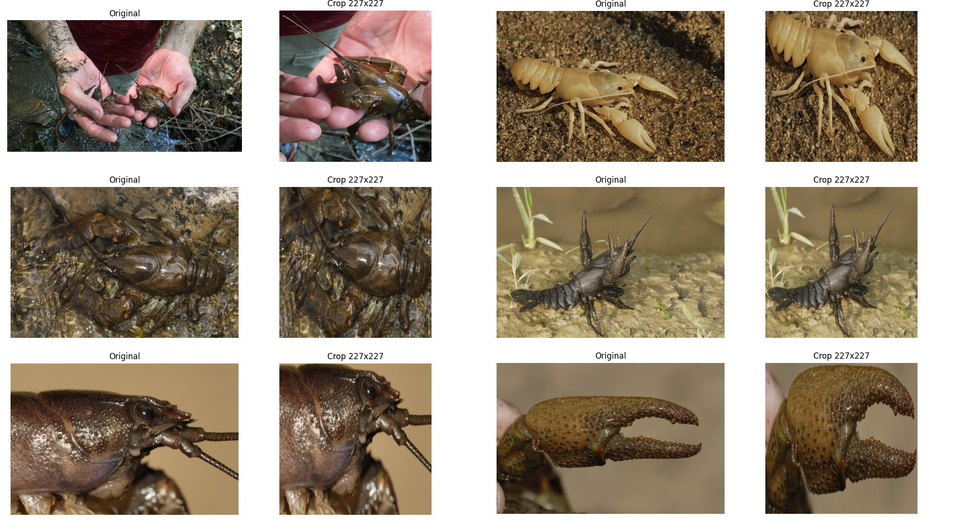
\includegraphics[width=\textwidth]{figs/torrentium_grid.png}
    \caption{Exemple din setul de date procesat pentru specia
    \textit{Austropotamobius torrentium}: imaginea originală (stânga)
    și regiunea de interes extrasă la rezoluția 227×227 pixeli (dreapta),
    pentru șase specimene reprezentative.}
    \label{fig:crop_torrentium}
\end{figure}
\begin{figure}[!htb]
    \centering
    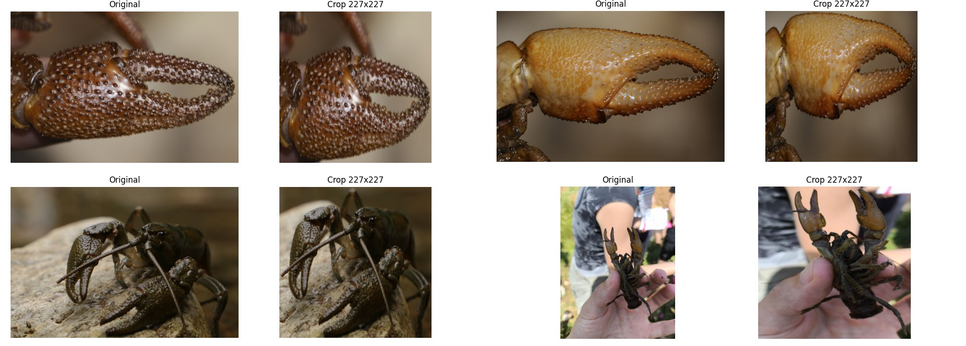
\includegraphics[width=\textwidth]{figs/bihariensis_grid.png}
    \caption{Exemple din setul de date procesat pentru specia
    \textit{Austropotamobius bihariensis}: imaginea originală (stânga)
    și regiunea de interes extrasă la rezoluția 227×227 pixeli (dreapta),
    pentru patru specimene reprezentative.}
    \label{fig:crop_bihariensis}
\end{figure}
\newpage


\section{Arhitectura modelului și transfer learning}

AlexNet \cite{krizhevsky2012imagenet} este o rețea neuronală convoluțională profundă compusă din cinci straturi convoluționale urmate de trei straturi complet conectate, proiectată inițial pentru clasificarea imaginilor din setul de date ImageNet pe 1000 de clase. În acest studiu, arhitectura este adaptată pentru clasificarea binară a celor două specii de rac, \textit{Austropotamobius bihariensis} și \textit{Austropotamobius torrentium}, prin tehnica transfer learning.




\subsection{Arhitectura AlexNet}

Imaginea de intrare are dimensiunea 227×227×3 pixeli. Deși  lucrarea originală \cite{krizhevsky2012imagenet} menționează o dimensiune de intrare de 224×224 pixeli, valoarea corectă din punct de vedere matematic, confirmată de dimensiunile hărților de caracteristici raportate în aceeași lucrare și utilizată în implementările moderne ale arhitecturii \cite{suh2018alexnet}, este de 227×227 pixeli. În consecință, toate imaginile din setul de date au fost redimensionate la 227×227 pixeli în etapa de preprocesare. Structura detaliată a arhitecturii este prezentată în Tabelul~\ref{tab:alexnet}.

\begin{table}[H]
\centering
\caption{Structura detaliată a arhitecturii AlexNet
\cite{krizhevsky2012imagenet}.}
\label{tab:alexnet}
\begin{tabular}{llcccc}
\hline
\textbf{Strat} & \textbf{Tip} & \textbf{Dimensiune ieșire} &
\textbf{Kernel} & \textbf{Pas} & \textbf{Activare} \\
\hline
Input   & Imagine      & 227×227×3   & --    & -- & --      \\
\hline
1       & Convoluție   & 55×55×96    & 11×11 & 4  & ReLU    \\
        & Max Pooling  & 27×27×96    & 3×3   & 2  & --      \\
\hline
2       & Convoluție   & 27×27×256   & 5×5   & 1  & ReLU    \\
        & Max Pooling  & 13×13×256   & 3×3   & 2  & --      \\
\hline
3       & Convoluție   & 13×13×384   & 3×3   & 1  & ReLU    \\
\hline
4       & Convoluție   & 13×13×384   & 3×3   & 1  & ReLU    \\
\hline
5       & Convoluție   & 13×13×256   & 3×3   & 1  & ReLU    \\
        & Max Pooling  & 6×6×256     & 3×3   & 2  & --      \\
\hline
6       & FC           & 4096        & --    & -- & ReLU    \\
7       & FC           & 4096        & --    & -- & ReLU    \\
8       & FC           & 1000        & --    & -- & Softmax \\
\hline
\end{tabular}
\end{table}





\subsection{Adaptarea prin transfer learning}

Ponderile straturilor convoluționale ale modelului AlexNet sunt inițializate cu valorile pre-antrenate pe setul de date ImageNet, care conține 1.2 milioane de imagini din 1000 de categorii vizuale diverse \cite{krizhevsky2012imagenet}. Aceste ponderi sunt menținute înghețate pe parcursul antrenării, adică nu sunt actualizate prin propagare inversă. Justificarea acestei alegeri constă în faptul că straturile convoluționale ale unui model pre-antrenat pe ImageNet învață reprezentări vizuale generale (muchii, texturi, forme) transferabile la domenii noi față de ImageNet, inclusiv la imaginile din domeniul biologiei acvatice.

Adaptarea modelului la problema de față constă în două intervenții. În primul rând, blocul convoluțional (\texttt{features}), compus din cele cinci straturi convoluționale și operațiile de max-pooling asociate, este înghețat: ponderile sale pre-antrenate pe ImageNet sunt menținute fixe pe parcursul întregului proces de antrenare și nu sunt actualizate prin propagare inversă. În al doilea rând, stratul de ieșire original (stratul FC 8), proiectat pentru 1000 de clase, este înlocuit cu un nou strat complet conectat cu 2 neuroni de ieșire, corespunzând celor două specii clasificate: \textit{Austropotamobius bihariensis} și \textit{Austropotamobius torrentium}. Straturile complet conectate FC 6 și FC 7, cu ponderile lor inițializate din ImageNet, sunt păstrate și ajustate (\textit{fine-tuned}) împreună cu noul strat de ieșire pe parcursul antrenării. În total, din cei 57.012.034 de parametri ai modelului, 2.469.696 (4,3\%) aparțin blocului convoluțional și rămân înghețați, iar 54.542.338 (95,7\%) sunt antrenabili, reprezentând întregul bloc al clasificatorului FC. Structura modificată este prezentată în Tabelul~\ref{tab:alexnet_adaptat}.

Dimensiunea straturilor FC 6 și FC 7 (4096 de neuroni fiecare) a fost păstrată identică cu arhitectura originală, deși acest nivel ascuns este neobișnuit de mare în raport cu dimensiunea redusă a stratului de ieșire (2 neuroni). Opțiunea a fost motivată de dorința de a exploata cât mai eficient ponderile pre-antrenate pe ImageNet ale acestor straturi. Pentru a evalua această decizie, a fost testată și o variantă alternativă a clasificatorului, cu un strat ascuns redus la 512 de neuroni (9216$\rightarrow$512$\rightarrow$2), inițializat aleatoriu și antrenat de la zero, fără a beneficia de ponderile pre-antrenate ale straturilor FC originale. Această variantă a obținut o acuratețe pe setul de testare de 91,84\%, inferioară configurației cu clasificator complet (4096 de neuroni, 95,92\%), confirmând că păstrarea dimensiunii originale a straturilor FC permite o valorificare mai eficientă a reprezentărilor învățate pe ImageNet, comparativ cu un clasificator mai mic, antrenat de la zero. Structura modificată a clasificatorului final este prezentată în Tabelul~\ref{tab:alexnet_adaptat}.

\begin{table}[H]
\centering
\caption{Structura AlexNet adaptată prin transfer learning pentru
clasificarea binară a speciilor de \textit{Austropotamobius}.}
\label{tab:alexnet_adaptat}
\begin{tabular}{llccc}
\hline
\textbf{Strat} & \textbf{Tip} & \textbf{Dimensiune ieșire} &
\textbf{Ponderi inițiale} & \textbf{Antrenat} \\
\hline
Input   & Imagine      & 227×227×3   & --           & --          \\
\hline
1       & Convoluție   & 55×55×96    & ImageNet     & Nu          \\
        & Max Pooling  & 27×27×96    & --           & --          \\
\hline
2       & Convoluție   & 27×27×256   & ImageNet     & Nu          \\
        & Max Pooling  & 13×13×256   & --           & --          \\
\hline
3       & Convoluție   & 13×13×384   & ImageNet     & Nu          \\
\hline
4       & Convoluție   & 13×13×384   & ImageNet     & Nu          \\
\hline
5       & Convoluție   & 13×13×256   & ImageNet     & Nu          \\
        & Max Pooling  & 6×6×256     & --           & --          \\
\hline
6       & FC           & 4096        & ImageNet     & \textbf{Da} \\
7       & FC           & 4096        & ImageNet     & \textbf{Da} \\
\hline
8       & FC           & 2           & Inițializare & \textbf{Da} \\
        &              &             & aleatorie    &             \\
\hline
\end{tabular}
\end{table}

Această abordare permite obținerea unor performanțe ridicate chiar și în condiții de eșantionare limitată, compensând dimensiunea redusă a setului de date disponibil (318 imagini) față de cerințele tipice ale antrenării de la zero a unei rețele convoluționale profunde \cite{krizhevsky2012imagenet}.






\section{Antrenarea modelului}\label{sec:antrenare}

\subsection{Împărțirea setului de date}

Setul de date procesat, conținând 318 imagini, este împărțit în trei subseturi disjuncte: antrenare, validare și testare. Împărțirea este realizată stratificat, separat pentru fiecare clasă, pentru a menține proporțiile originale ale distribuției în toate cele trei subseturi. Rapoartele utilizate sunt 70\% pentru antrenare, 15\% pentru validare și 15\% pentru testare, rezultând distribuția prezentată în Tabelul~\ref{tab:split}.

\begin{table}[H]
\centering
\caption{Distribuția imaginilor pe subseturi de antrenare, validareși testare.}
\label{tab:split}
\begin{tabular}{lcccc}
\hline
\textbf{Specie} & \textbf{Total} & \textbf{Antrenare} &
\textbf{Validare} & \textbf{Testare} \\
\hline
\textit{A. bihariensis} & 182 & 127 & 27 & 28 \\
\textit{A. torrentium}  & 136 & 95  & 20 & 21 \\
\hline
\textbf{Total}          & 318 & 222 & 47 & 49 \\
\hline
\end{tabular}
\end{table}

Reproductibilitatea împărțirii este asigurată prin fixarea unei semințe aleatoare (\textit{random seed}) cu valoarea 42, aplicată consistent pentru generatoarele de numere aleatoare din bibliotecile Python, NumPy și PyTorch.

\subsection{Augmentarea datelor de antrenare}

Datorită dimensiunii reduse a setului de antrenare (222 de imagini), este aplicat un set extins de tehnici de augmentare la runtime, exclusiv pe datele de antrenare. Seturile de validare și testare nu sunt supuse augmentării, conținând doar imaginile originale preprocesate, pentru a asigura o evaluare obiectivă a performanței modelului. Tehnicile de augmentare aplicate sunt prezentate în Tabelul~\ref{tab:augmentare}.

\begin{table}[H]
\centering
\caption{Tehnicile de augmentare aplicate la runtime pe setul de antrenare.}
\label{tab:augmentare}
\begin{tabular}{lp{7cm}}
\hline
\textbf{Tehnică} & \textbf{Parametri} \\
\hline
Oglindire orizontală    & Probabilitate 0.5 \\
Oglindire verticală     & Probabilitate 0.3 \\
Rotație aleatorie       & Unghi maxim ±45° \\
Deformare perspectivă   & Scală distorsiune 0.3, probabilitate 0.4 \\
Crop aleatoriu          & Scală 80--100\%, raport aspect 0.9--1.1 \\
Variație culoare        & Luminozitate 0.4, contrast 0.4,
                          saturație 0.3, nuanță 0.1 \\
Conversie tonuri de gri & Probabilitate 0.1 \\
Blur gaussian           & Kernel 3×3, $\sigma \in [0{.}1,\ 2{.}0]$ \\
Ștergere aleatorie      & Probabilitate 0.3, scală 2--15\%
                          din suprafața imaginii \\
\hline
\end{tabular}
\end{table}

Figura~\ref{fig:augmentari_bihariensis} și Figura~\ref{fig:augmentari_torrentium} ilustrează imaginea originală și opt variante augmentate ale aceleiași imagini, pentru câte un specimen din fiecare specie, generate prin aplicarea succesivă a tehnicilor prezentate în Tabelul~\ref{tab:augmentare}. Deasupra fiecărei variante sunt indicate tehnicile activate efectiv la acea rulare, dat fiind caracterul stocastic al augmentării (fiecare tehnică se activează independent, pe baza probabilității proprii).

\begin{figure}[htbp]
    \centering
    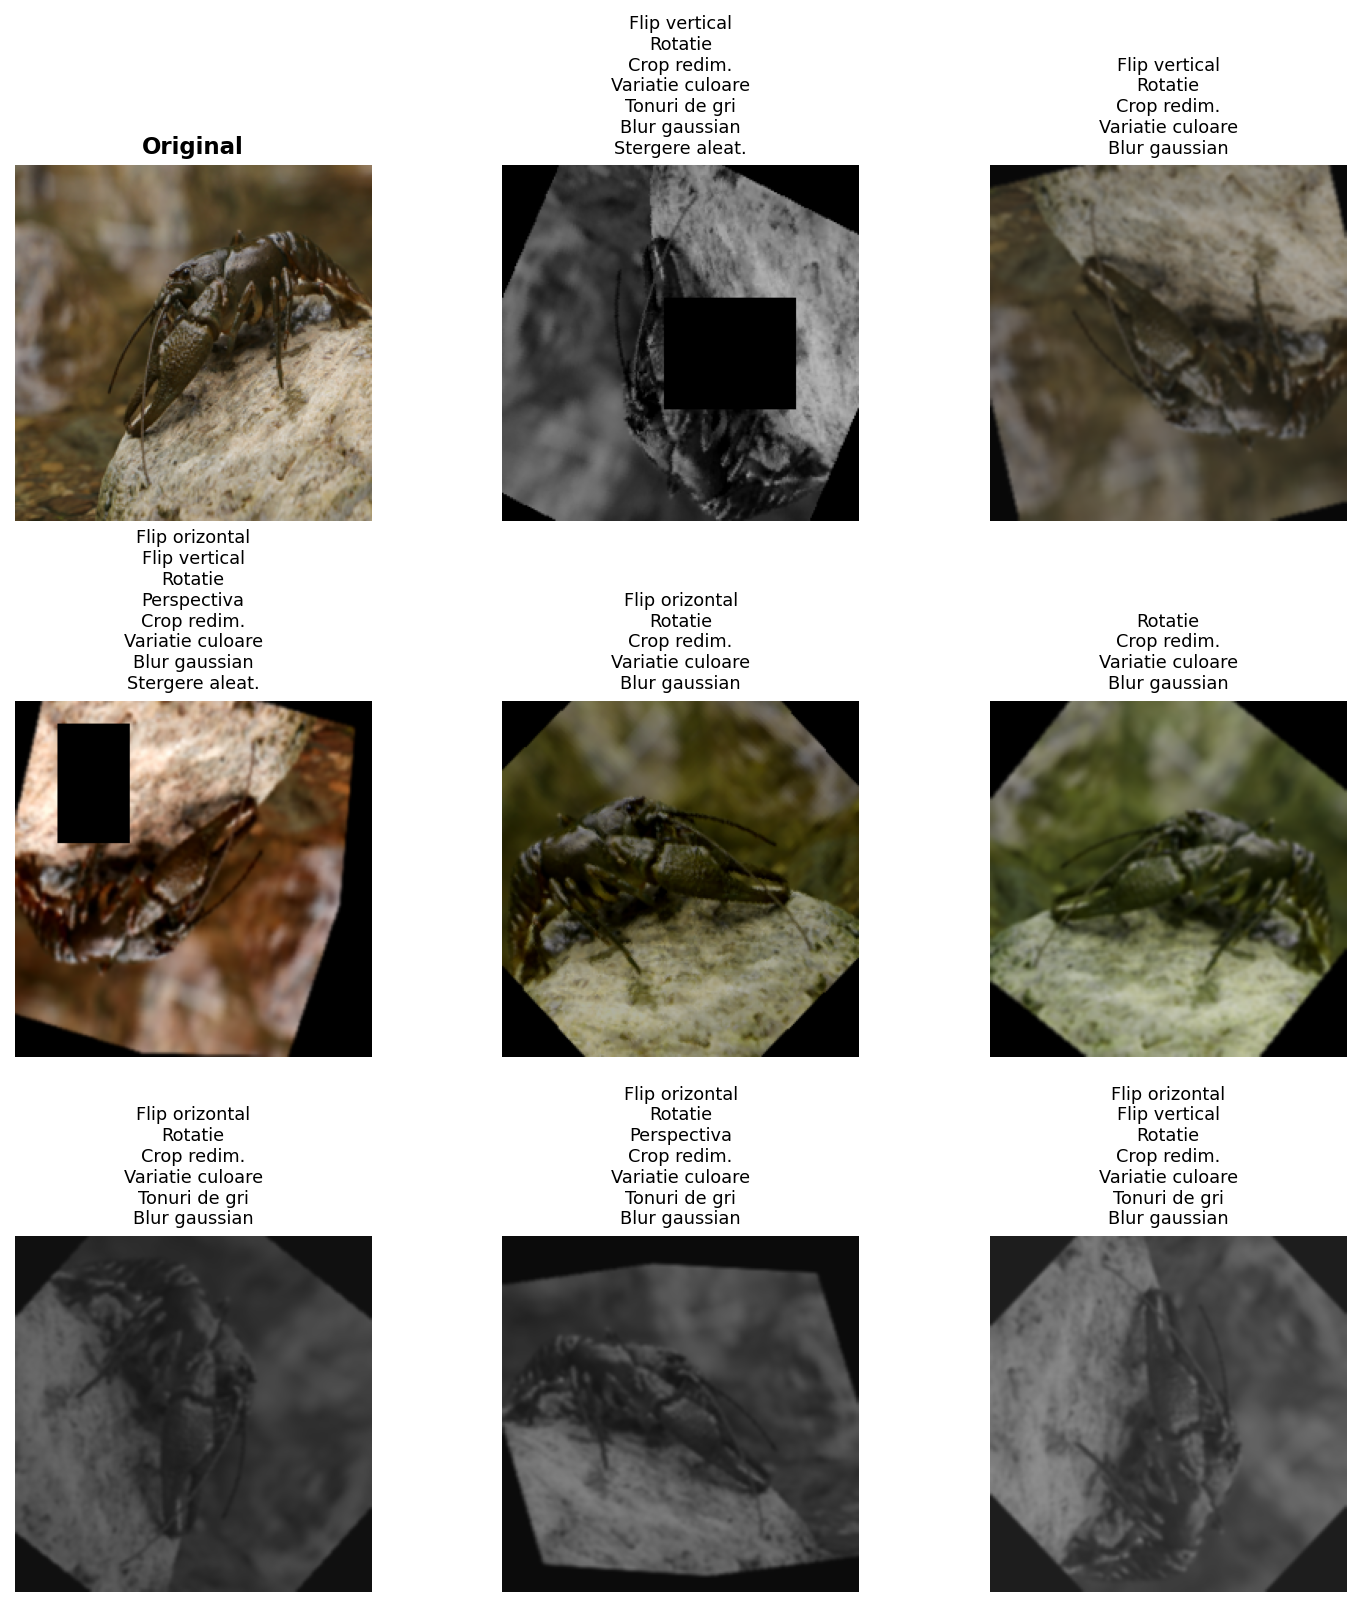
\includegraphics[width=\textwidth]{figs/AugmentariGridBihariensis.png}
    \caption{Imaginea originală și opt variante augmentate ale unui
    specimen de \textit{Austropotamobius bihariensis}, cu tehnicile
    aplicate la fiecare rulare indicate deasupra imaginii
    corespunzătoare.}
    \label{fig:augmentari_bihariensis}
\end{figure}

\begin{figure}[htbp]
    \centering
    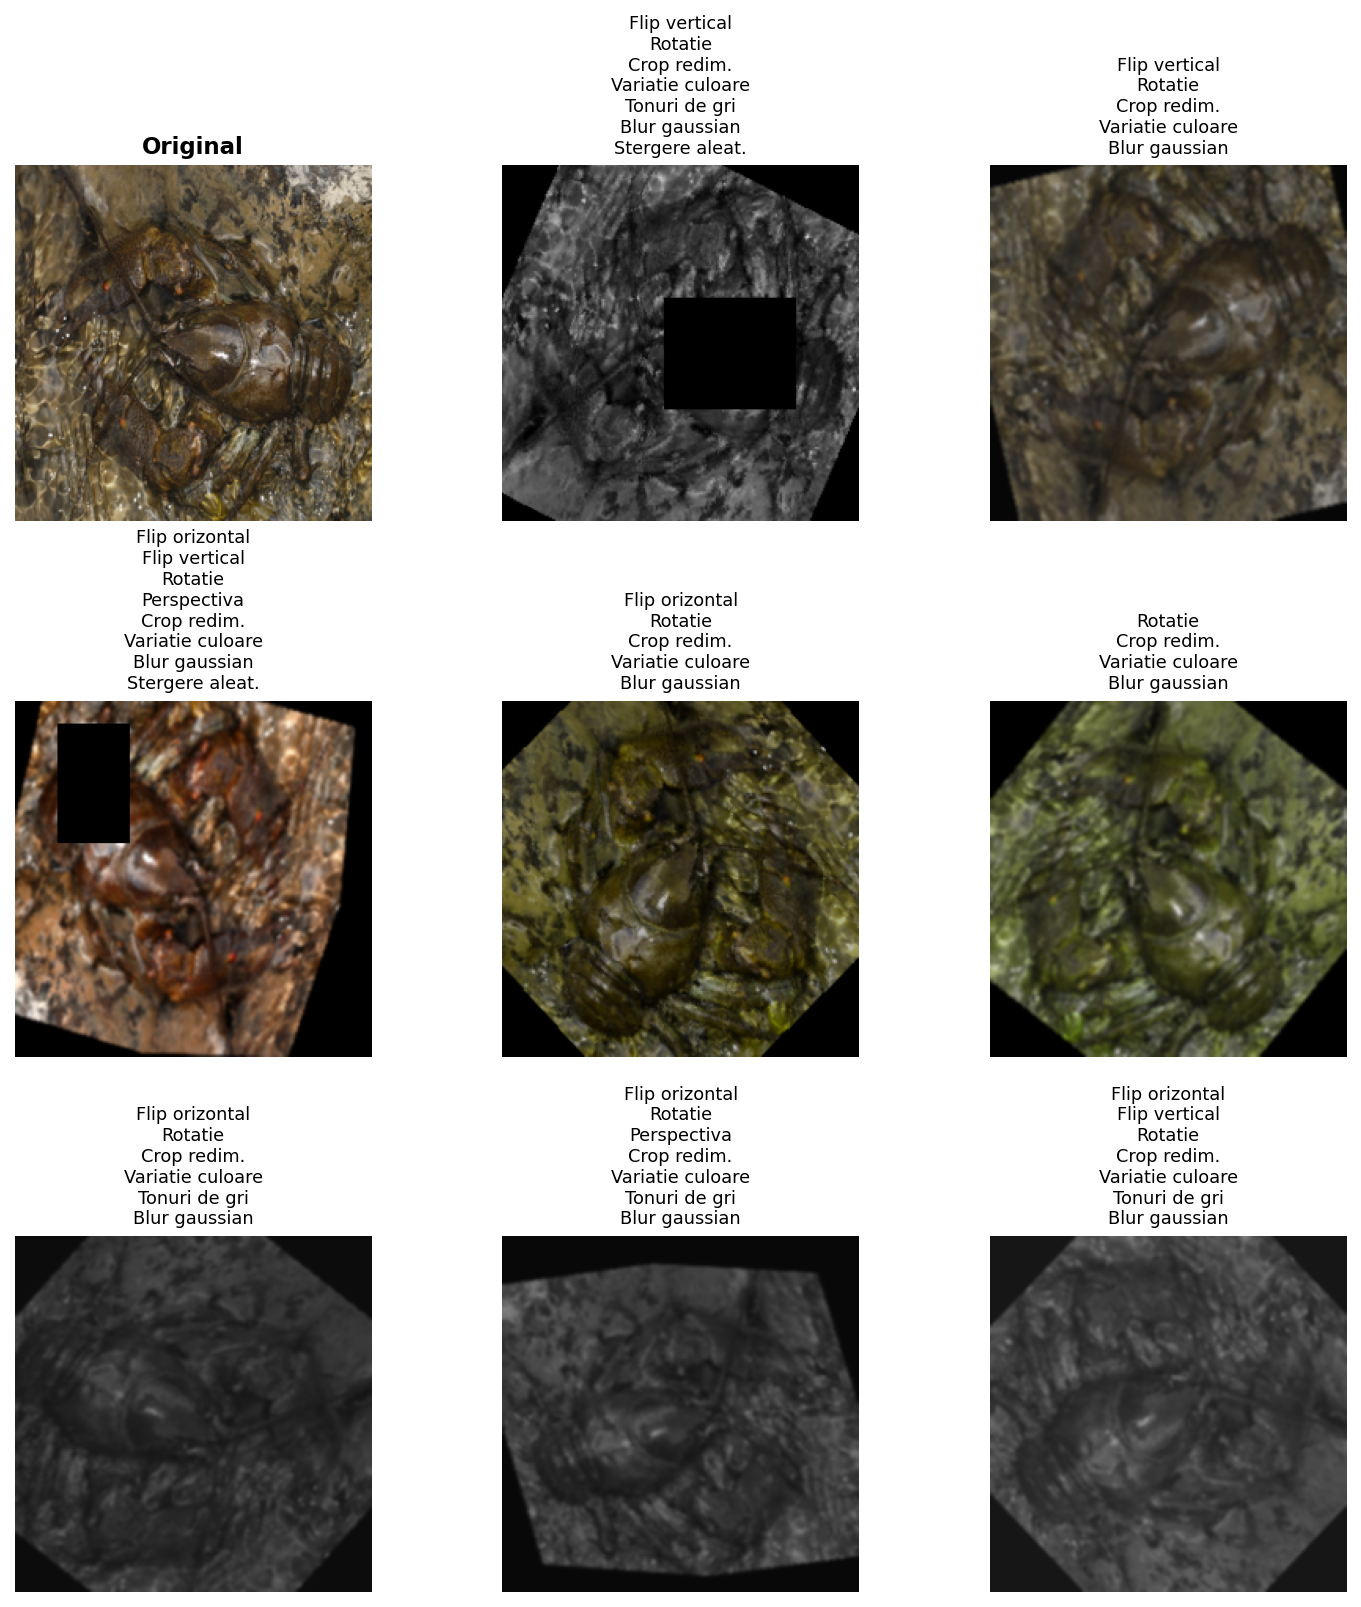
\includegraphics[width=\textwidth]{figs/AugmentariGridTorrentium.png}
    \caption{Imaginea originală și opt variante augmentate ale unui
    specimen de \textit{Austropotamobius torrentium}, cu tehnicile
    aplicate la fiecare rulare indicate deasupra imaginii
    corespunzătoare.}
    \label{fig:augmentari_torrentium}
\end{figure}



\subsection{Normalizarea datelor}

Toate imaginile, indiferent de subset, sunt normalizate cu media și deviația standard calculate pe setul de date ImageNet: $\mu = [0{,}485,\ 0{,}456,\ 0{,}406]$ și $\sigma = [0{,}229,\ 0{,}224,\ 0{,}225]$, care corespund canalelor RGB. Această normalizare este necesară pentru compatibilitatea cu ponderile pre-antrenate ale modelului AlexNet, care au fost obținute pe date procesate cu aceleași constante \cite{krizhevsky2012imagenet}.

\subsection{Configurația antrenării}

Antrenarea este realizată pe 60 de epoci cu un batch size de 32 de imagini. Funcția de pierdere utilizată este Cross-Entropy Loss cu Label Smoothing de 0.1, aplicat pentru a reduce supra-încrederea modelului  în predicțiile sale (\textit{overconfidence}) și a îmbunătăți generalizarea pe seturi de date mici.

Optimizatorul utilizat este SGD (\textit{Stochastic Gradient Descent}) cu coeficient pentru termenul momentum egal cu 0.9, rată de învățare inițială 0.001 și weight decay 0,0005. Rata de învățare este ajustată automat printr-un planificator (\textit{scheduler}) de tip \textit{ReduceLROnPlateau}, care reduce rata de învățare cu un factor de 0.1 atunci când pierderea pe setul de validare nu se îmbunătățește timp de 10 epoci consecutive.

Selecția modelului final se face pe baza celei mai bune valori a acurateții obținute pe setul de validare pe parcursul antrenării, ponderile corespunzătoare fiind salvate și utilizate ulterior pentru evaluarea pe setul de testare. Configurația completă a hiperparametrilor este prezentată în Tabelul~\ref{tab:hiperparametri}.

\begin{table}[H]
\centering
\caption{Configurația hiperparametrilor utilizați în antrenare.}
\label{tab:hiperparametri}
\begin{tabular}{lc}
\hline
\textbf{Hiperparametru} & \textbf{Valoare} \\
\hline
Număr epoci          & 60 \\
Batch size           & 32 \\
Rată de învățare     & 0.001 \\
Momentum             & 0.9 \\
Weight decay         & 0.0005 \\
Label smoothing      & 0.1 \\
Optimizer            & SGD \\
Scheduler            & ReduceLROnPlateau \\
Factor reducere LR   & 0.1 \\
Răbdare scheduler    & 10 epoci \\
Random seed          & 42 \\
\hline
\end{tabular}
\end{table}








\section{Evaluarea performanței}

Performanța modelului a fost evaluată pe setul de testare, format din 49 de imagini nevăzute de model în timpul antrenării (28 de specimene de \textit{Austropotamobius bihariensis} și 21 de specimene de \textit{Austropotamobius torrentium}). Metrica principală utilizată este acuratețea pe setul de testare, calculată ca raport între numărul de predicții corecte și numărul total de exemple din setul de test.

Pentru o evaluare mai detaliată a performanței pe fiecare clasă, au fost calculate suplimentar metricile precizie (\textit{precision}), rata de regăsire (\textit{recall}) și scorul F1 (\textit{F1-score}), pe baza matricei de confuzie prezentate în Tabelul~\ref{tab:confuzie}.

\begin{table}[H]
\centering
\caption{Matricea de confuzie pe setul de testare.}
\label{tab:confuzie}
\begin{tabular}{lcc}
\hline
\textbf{Specia reală} & \textbf{Prezis \textit{bihariensis}} & \textbf{Prezis \textit{torrentium}} \\
\hline
\textit{A. bihariensis} & 27 & 1 \\
\textit{A. torrentium}  & 1  & 20 \\
\hline
\end{tabular}
\end{table}

Tabelul~\ref{tab:metrici} prezintă precizia, rata de regăsire și scorul F1 calculate pentru fiecare clasă în parte.

\begin{table}[H]
\centering
\caption{Precizia, rata de regăsire și scorul F1 pe fiecare clasă.}
\label{tab:metrici}
\begin{tabular}{lccc}
\hline
\textbf{Specia} & \textbf{Precizie} & \textbf{Recall} & \textbf{F1-score} \\
\hline
\textit{A. bihariensis} & 0.9643 & 0.9643 & 0.9643 \\
\textit{A. torrentium}  & 0.9524 & 0.9524 & 0.9524 \\
\hline
\end{tabular}
\end{table}

Valorile apropiate ale celor trei metrici pentru ambele clase confirmă un comportament echilibrat al modelului, fără o tendință sistematică de a favoriza o specie în detrimentul celeilalte. Scorul F1 mediu (macro-mediu) obținut este de 0,9583.

Modelul final a fost obținut printr-un proces iterativ de rafinare, în care fiecare etapă a adus îmbunătățiri măsurabile față de configurația anterioară. Evoluția acurateții pe setul de testare de-a lungul celor patru configurații experimentate este prezentată în Tabelul~\ref{tab:evolutie_runs}.

\begin{table}[H]
\centering
\caption{Evoluția acurateții pe setul de testare în funcție de
configurația experimentată.}
\label{tab:evolutie_runs}
\begin{tabular}{cp{9cm}c}
\hline
\textbf{Configurație} & \textbf{Modificări față de configurația anterioară}
& \textbf{Acuratețe test} \\
\hline
1 & Split stratificat 70/15/15, fără alte intervenții & 62.50\% \\
2 & + Înghețare convoluții, normalizare ImageNet, augmentări, seed fix & 87.50\% \\
3 & + Extragere regiuni de interes (crop cu LabelMe) & \textbf{95.92\%} \\
4 & Identic cu configurația 3, batch size 64 & 93.88\% \\
\hline
\end{tabular}
\end{table}

Prima configurație, folosind exclusiv împărțirea stratificată a datelor fără nicio altă intervenție, a produs o acuratețe de 62,50\% pe setul de testare, cu puțin peste nivelul unei clasificări aleatorii binare, indicând că modelul nu reușea să extragă trăsături discriminante relevante din imaginile brute neadnotate.

Introducerea în celei de-a doua configurații a înghețării blocului convoluțional, a normalizării ImageNet, a augmentărilor la runtime și a fixării semințelor aleatoare a adus un salt semnificativ la 87,50\%, confirmând că transferul de cunoștințe din ImageNet este eficient chiar și pe un set de date de dimensiune redusă, cu condiția ca datele de intrare să fie compatibile cu formatul așteptat de model.

Cel mai important salt de performanță a fost produs de introducerea extragerii automate a regiunilor de interes pe baza adnotărilor LabelMe. Prin eliminarea fondului irelevant (substrat acvatic, vegetație, mâini ale colectorului) și centrarea imaginii pe specimenul de interes, modelul a avut acces la trăsăturile morfologice discriminante ale celor două specii, ceea ce a condus la o acuratețe de 95,92\% în cea de-a treia configurație. Extragerea regiunilor de interes a fost aplicată uniform pe toate cele trei subseturi (antrenare, validare și testare), înainte de împărțirea stratificată a datelor, astfel încât evaluarea pe setul de testare să reflecte fidel performanța modelului pe imagini deja procesate prin același flux.

Creșterea dimensiunii batch-ului la 64 în cea de-a patra configurație a dus la o ușoară scădere a acurateței la 93,88\%, sugerând că un batch size mai mic favorizează generalizarea în contextul unui set de antrenare de dimensiuni reduse (222 de imagini). Modelul reținut ca rezultat final al lucrării corespunde configurației 3, cu o acuratețe pe setul de testare de \textbf{95,92\%}.


% detalii privind construirea setului de date